\chapter{Arhitektura i dizajn sustava}

    \begin{figure}[!h]
		\centering
		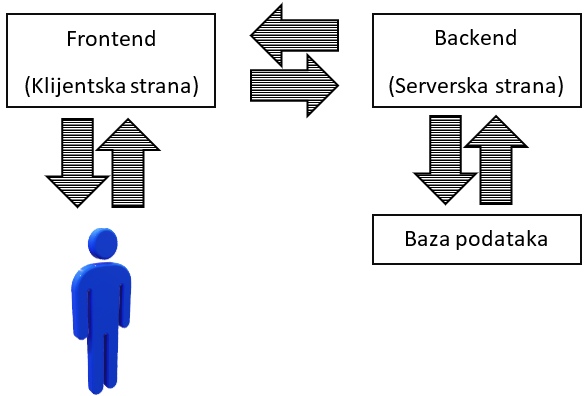
\includegraphics[width=13cm]{slike/arhitektura.PNG} 
		\caption{Arhitektura sustava}
		\label{fig:arhitektura}
	\end{figure}

	Korisnik aplikaciji pristupa putem web preglednika. Interakciju s aplikacijom ostvaruje preko korisničkog sučelja pomoću kojeg šalje zahtjeve web poslužitelju i prima odgovore.\\
Programski jezik pomoću kojeg je ostvaren backend web aplikacije je Java, a korišteni radni okvir je Spring Boot. Frontend aplikacije ostvaren je programskim jezikom JavaScript i bibliotekom React.js. Za razvojno okruženje odabran je Intellij IDEA. Spring Boot je radni okvir namijenjen stvaranju mikroservisa. Mikroservis je arhitektura koja omogućuje neovisan razvoj više različitih servisa od kojih svaki ima svoj proces.\\
Web aplikaciju čine tri osnovna dijela:
	\begin{itemize}
		\item 	\textbf{frontend}
		\item 	\textbf{backend}
		\item 	\textbf{baza podataka }		
	\end{itemize}
Frontend se sastoji od komponenata i logike. Istu komponentu je moguće koristiti za različite namjene (engl. reusability). React.js koristi virtualni DOM (engl. Document Object Model) čiji se sadržaj uspoređuje sa stvarnim DOM-om i na osnovu toga se provode promjene što za posljedicu ima poboljšanje performansi. Struktura ostvarena međusobnim povezivanjem različitih komponenti je stablo.\\
Backend se sastoji od: 
\begin{itemize}
		\item 	programskog sučelja za reprezentacijski prijenos stanja (REST API), odnosno Controller-a
		\item 	sloja poslovne logike (Service)
		\item 	sloja za pristup bazi podataka (Repository)		
	\end{itemize}
\textbf{Controller} izlaže funkcionalnost web aplikacije kao RESTful web usluge, tj. prima zahtjeve čiji su glavni dijelovi URI, metoda i HTTP zaglavlje, a korisniku šalje odgovor koji se sastoji od statusnog koda, tijela poruke i zaglavlja. U tijelu poruke se nalazi sadržaj kojeg korisnik konzumira nakon što je prikazan u web pregledniku. Komunikaciju sa slojem poslovne logike Controller ostvaruje pomoću umetanja ovisnosti (engl. dependency injection). Dependency injection je obrazac prema kojemu se u određeni objekt/funkciju umeće neki drugi objekt/funkcija na koji se prvobitno spomenuti objekt/funkcija oslanja.\\
\textbf{Service} omogućuje komunikaciju između slojeva Controller i Repository, zadužen je za provjeru ispravnosti podataka. Osim na sloju Service, provjera ispravnosti se obavlja na frontend-u i u bazi podataka. Komunikaciju sa slojem za pristup bazi podataka ostvaruje umetanjem ovisnosti.\\ 
\textbf{Repository} omogućuje komunikaciju s bazom podataka pomoću SQL-a. Objekti iz relacijske baze podataka pretvaraju se objekte programskog jezika Java korištenjem tehnike ORM.\\\\
		

				
		\section{Baza podataka}

		Baza podataka za aplikaciju implementirana je u obliku relacijske baze podataka, koja podatke sprema u obliku redaka ili n-torki i stupaca ili atributa koji zajedno tvore tablicu.  \\
Glavna komponenta baze je tablica Korisnik, koja se puni osobnim podacima unesenim pri registraciji u sustav.  Svakom novom korisniku dodjeljuje se primarni ključ, unikatan identifikacijski broj pomoću kojeg se korisnici u bazi podataka međusobno razlikuju. Budući da korisnik ima jednu ili više dodijeljenih uloga, koje su definirane u tablici Uloga, izrađena je veza između dvije tablice koja sadrži identifikacijske brojeve korisnika i odgovarajuće uloge. \\
Kako bi korisnik zaigrao na kvizu, potrebno je prvo pronaći ekipu kojoj odgovara svojim područjima znanja, zbog čega je izrađena tablica Ekipa koja sadrži minimalno jednoga, a maksimalno petero članova.  \\
Ako korisnik ima ulogu sastavljača, on kreira kviz s podacima i informacijama koji se spremaju u tablicu Kviz.  Svaki kviz ima svoj identifikacijski broj i unikatne atribute, vrijeme održavanja i ID sastavljača, jer jedan sastavljač ne može objaviti dva različita kviza koja se održavaju u isto vrijeme.  \\
Tablica Obavijest sadrži svoj identifikacijski broj, tekst obavijesti koji se prikazuje korisniku i ID korisnika kao strani ključ. \\

		
			\subsection{Opis tablica}
				
			
				\begin{longtblr} [
					label = none,
					entry = none
					] {
						width = \textwidth,
						colspec = {|X[8,l]|X[8, l]|X[16, l]|},
						rowhead = 1,
					}
					\hline \textbf{Korisnik} & \\ \hline[3pt]
					\SetCell{LightGreen}korisnik\_id & BIG INT & Identifikacijski broj korisnika, primarni ključ.\\ \hline
					ime & VARCHAR(100) & Ime korisnika. \\ \hline
					prezime & VARCHAR(100) & Prezime korisnika. \\ \hline
					email\_adresa(U) & VARCHAR(100) & E-mail adresa korisnika. \\ \hline
					lozinka & VARCHAR(50) & Lozinka koju korisnik osmisli pri registraciji. \\ \hline
					slika & VARBINARY & Profilna slika korisnika u aplikaciji, opcionalno. \\ \hline
					broj\_telefona & VARCHAR(50) & Broj telefona korisnika, opcionalno. \\ \hline
					podrucja\_znanja & VARCHAR(150) & Područja znanja igrača, koriste se pri odabiru ekipe. \\ \hline
					nadimak(U) & VARCHAR(50) & Nadimak koji si korisnik osmisli pri registraciji. \\ \hline
					prosj\_broj\_ekipa & INT & Prosječan broj ekipa koji sudjeluju u kvizovima nekog sastavljača, opcionalno. \\ \hline
					blokiran & BOOLEAN & Atribut koji daje informaciju o tome je li korisnik blokiran ili ne. \\ \hline
					\SetCell{LightBlue}ekipa\_id & BIG INT & Identifikacijski broj ekipe kojoj korisnik pripada, opcionalno. \\ \hline
				\end{longtblr}

				\begin{longtblr}[
					label = none,
					entry = none
				]{
					width = \textwidth,
					colspec = {|X[8,l]|X[8, l]|X[16, l]|},
					rowhead = 1,
                         		}
				\hline \textbf{Uloga} & \\ \hline[3pt]
				\SetCell{LightGreen} uloga\_id & BIG INT & Identifikacijski broj uloge. \\ \hline
				uloga\_ime & VARCHAR(50) & Ime uloge. \\ \hline
				\end{longtblr}



			
				\begin{longtblr}[
					label = none, 
					entry = none
					]{
						width = \textwidth,
						colspec = {|X[8,l]|X[8, l]|X[16, l]|},
						rowhead = 1,
					}
					\hline \textbf{korisnik\_uloga} & \\ \hline[3pt]
					\SetCell{LightBlue} uloga\_id & BIG INT & Identifikacijski broj uloge, strani ključ s referencom na ulogu.\\ \hline
					\SetCell{LightBlue} korisnik\_id & BIG INT & Identifikacijski broj korisnika, strani ključ s referencom na korisnika. \\ \hline
				\end{longtblr}
			
				\begin{longtblr} [
					label = none, 
					entry = none
					]{
						width = \textwidth,
						colspec = {|X[8,l]|X[8, l]|X[16, l]|},
						rowhead = 1,
					}
					\hline \textbf{Ekipa} & \\ \hline[3pt]
					\SetCell{LightGreen} ekipa\_id & BIG INT & Identifikacijski broj ekipe, primarni ključ. \\ \hline
					broj\_clanova & INT & Broj članova ekipe, ne smije biti manji od 1 ni veći od 5. \\ \hline
					naziv\_ekipe(U) & VARCHAR(50) & Ime ekipe. \\ \hline
				\end{longtblr}
			
			\begin{longtblr} [
				label = none,
				entry = none
				]{
					width = \textwidth,
					colspec = {|X[8,l]|X[8, l]|X[16, l]|},
					rowhead = 1,
				}
			\hline \textbf{Kviz} & \\ \hline[3pt]
			\SetCell{LightGreen} kviz\_id & BIG INT & Identifikacijski broj kviza, primarni ključ. \\ \hline
			kratki\_opis & VARCHAR(200) & Sažeti tekst o sadržaju kviza. \\ \hline
			ime\_kafica & VARCHAR(50) & Ime kafića u kojem se kviz održava. \\ \hline
			vrijeme\_odrzavanja (U) & TIMESTAMP & Vrijeme održavanja kviza, unikatan atribut zajedno s identifikacijskim brojem sastavljača. \\ \hline
			lokacija & GEOGRAPHY & Lokacija mjesta održavanja. \\ \hline
			maks\_broj\_ekipa & INT & Maksimalni broj ekipa koje sudjeluju na kvizu. \\ \hline
			kotizacija & FLOAT & Kotizacija za sudjelovanje na kvizu. \\ \hline
			nagrade & VARCHAR(100) & Popis nagrada na visoko plasirane ekipe. \\ \hline
			vrsta & VARCHAR(50) & Vrsta kviza (povijest, sport, ..). \\ \hline
			naziv\_kviza (U) & VARCHAR(50) & Unikatan naziv kviza. \\ \hline
			aktivan & BOOLEAN & Predstavlja je li kviz trenutno aktivan ili ne. \\ \hline
			\SetCell{LightBlue} korisnik\_id & BIG INT & Identifikacijski broj sastavljača, strani ključ s referencom na korisnika. \\ \hline
			\end{longtblr}

			

			\begin{longtblr}[
				label = none,
				entry = none
			]{
				width = \textwidth,
				colspec = {|X[8,l]|X[8, l]|X[16, l]|},
				rowhead = 1,
			}
			\hline \textbf{sudjeluje\_u} & \\ \hline[3pt]
			\SetCell{LightBlue} ekipa\_id & BIG INT & Identifikacijski broj ekipe, strani ključ s referencom na ekipu. \\ \hline
			\SetCell{LightBlue} kviz\_id & BIG INT & Identifikacijski broj kviza na kojem sudjeluje ekipa, strani ključ. \\ \hline
			\end{longtblr}

			\begin{longtblr} [
				label = none,
				entry = none
			]{
				width = \textwidth,
				colspec = {|X[8,l]|X[8, l]|X[16, l]|},
				rowhead = 1,
			}
			\hline \textbf{Obavijest}& \\ \hline[3pt]
			\SetCell{LightGreen} obavijest\_id & BIG INT & Identifikacijski broj obavijesti, primarni ključ. \\ \hline
			tekst & VARCHAR(300) & Tekst obavijesti. \\ \hline
			\SetCell{LightBlue} korisnik\_id & BIG INT & Identifikacijski broj korisnika koji je primio obavijest. \\ \hline
			\end{longtblr}
			
			
				
				
			
			\subsection{Dijagram baze podataka}
			 \begin{figure}[!h]
			\centering
			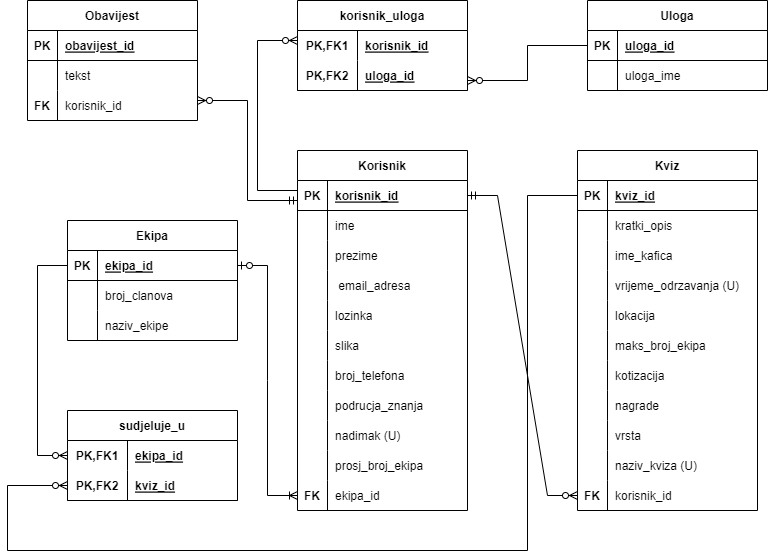
\includegraphics[width=15cm]{slike/final.png} 
			\caption{ER dijagram}
			\label{fig:arhitektura}
	\end{figure}
			
			\eject
			
			
		\section{Dijagram razreda}
		
			\begin{figure}[H]
				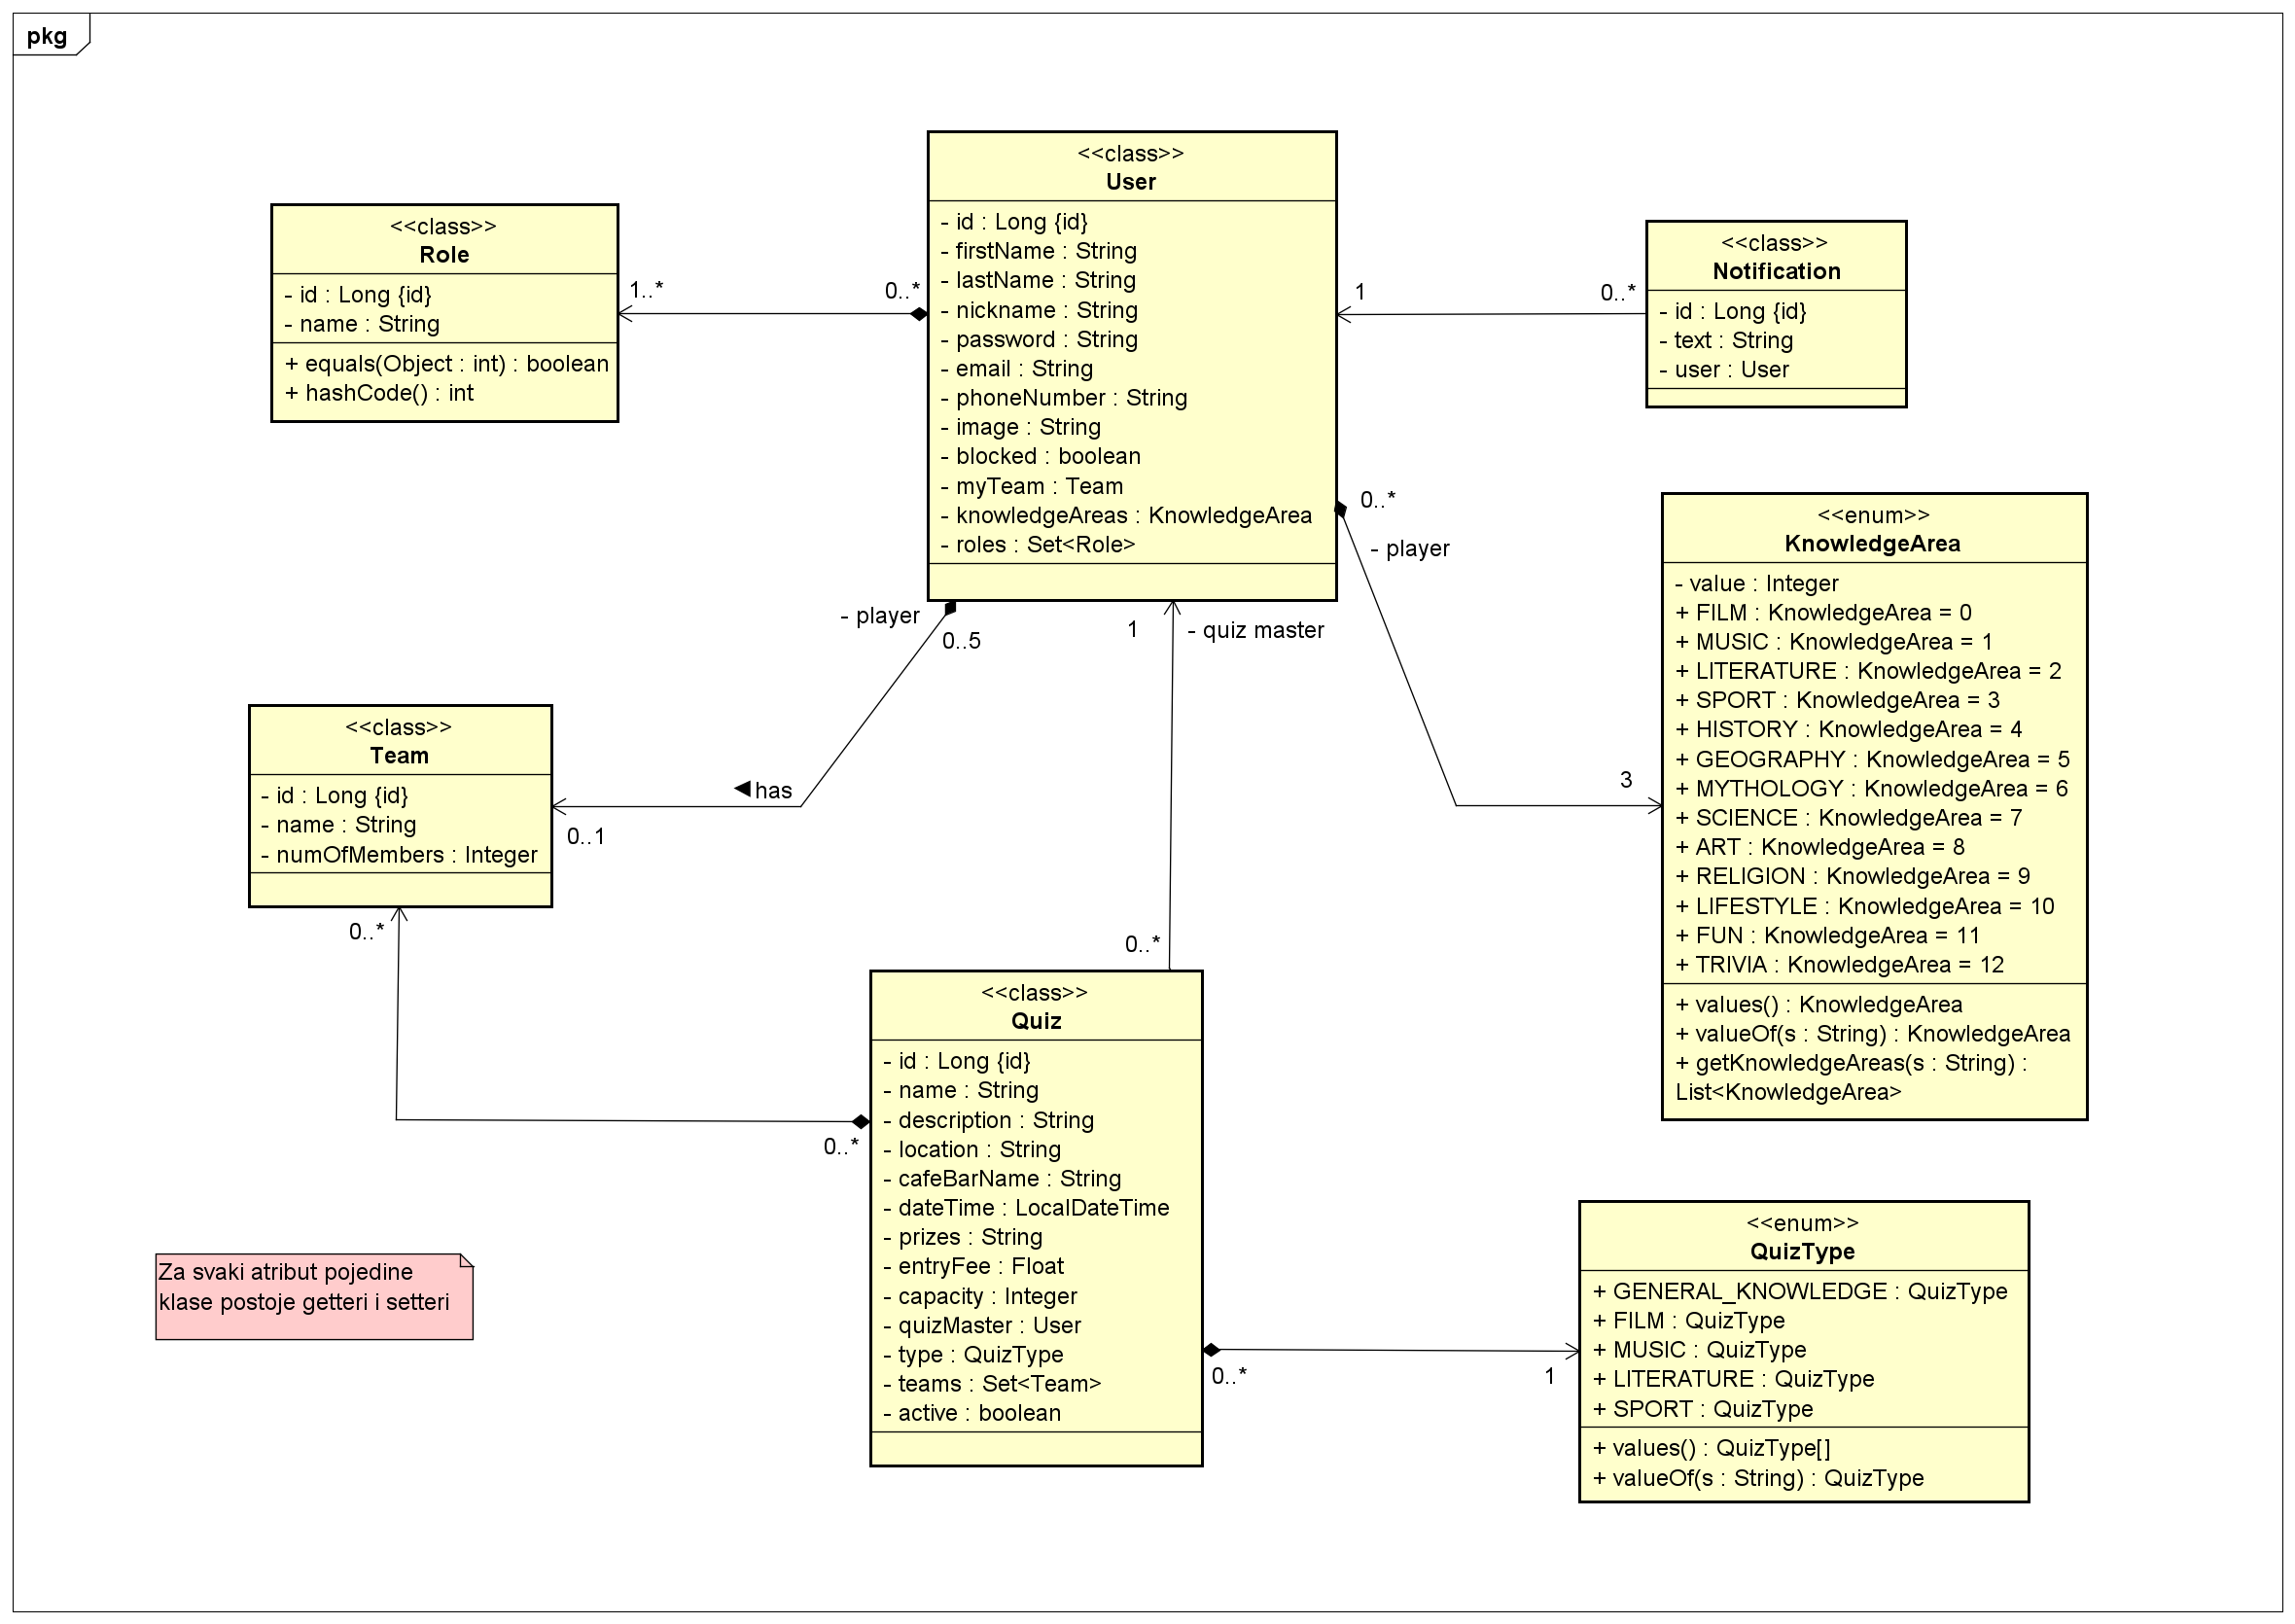
\includegraphics[width=\textwidth]{dijagrami/classDiagram1.PNG} 
				\caption{Dijagram razreda, dio Modeli}
				\label{fig:classDiagram1}
			\end{figure}
		
			Na slici 4.3 prikazan je dijagram razreda koji prikazuje razrede u objektno orijentiranom sustavu, njihove atribute i metode te međusobnu povezanost. Model razreda preslikava se u bazu podataka prema načelu ORM-a. Razred User predstavlja registriranog korisnika aplikacije koji može imati jednu ili više uloga opisane razredom Role. Korisnik prima obavijesti predstavljene razredom Notification, a kao igrač može pripadati najviše jednoj ekipi koja je opisana razredom Team. Također, korisnik koji je igrač izabire točno tri područja znanja koja su u aplikaciji ostvarena kao enumeracija KnowledgeArea. Korisnik koji je sastavljač može kreirati neograničen broj kvizova opisanih razredom Quiz, a svaki je kviz točno jedne vrste predstavljene enumeracijom QuizType te na jednom kvizu sudjeluje više ekipa, čiji je maksimalni broj određen atributom capacity razreda Quiz. 
			
			\begin{figure}[H]
				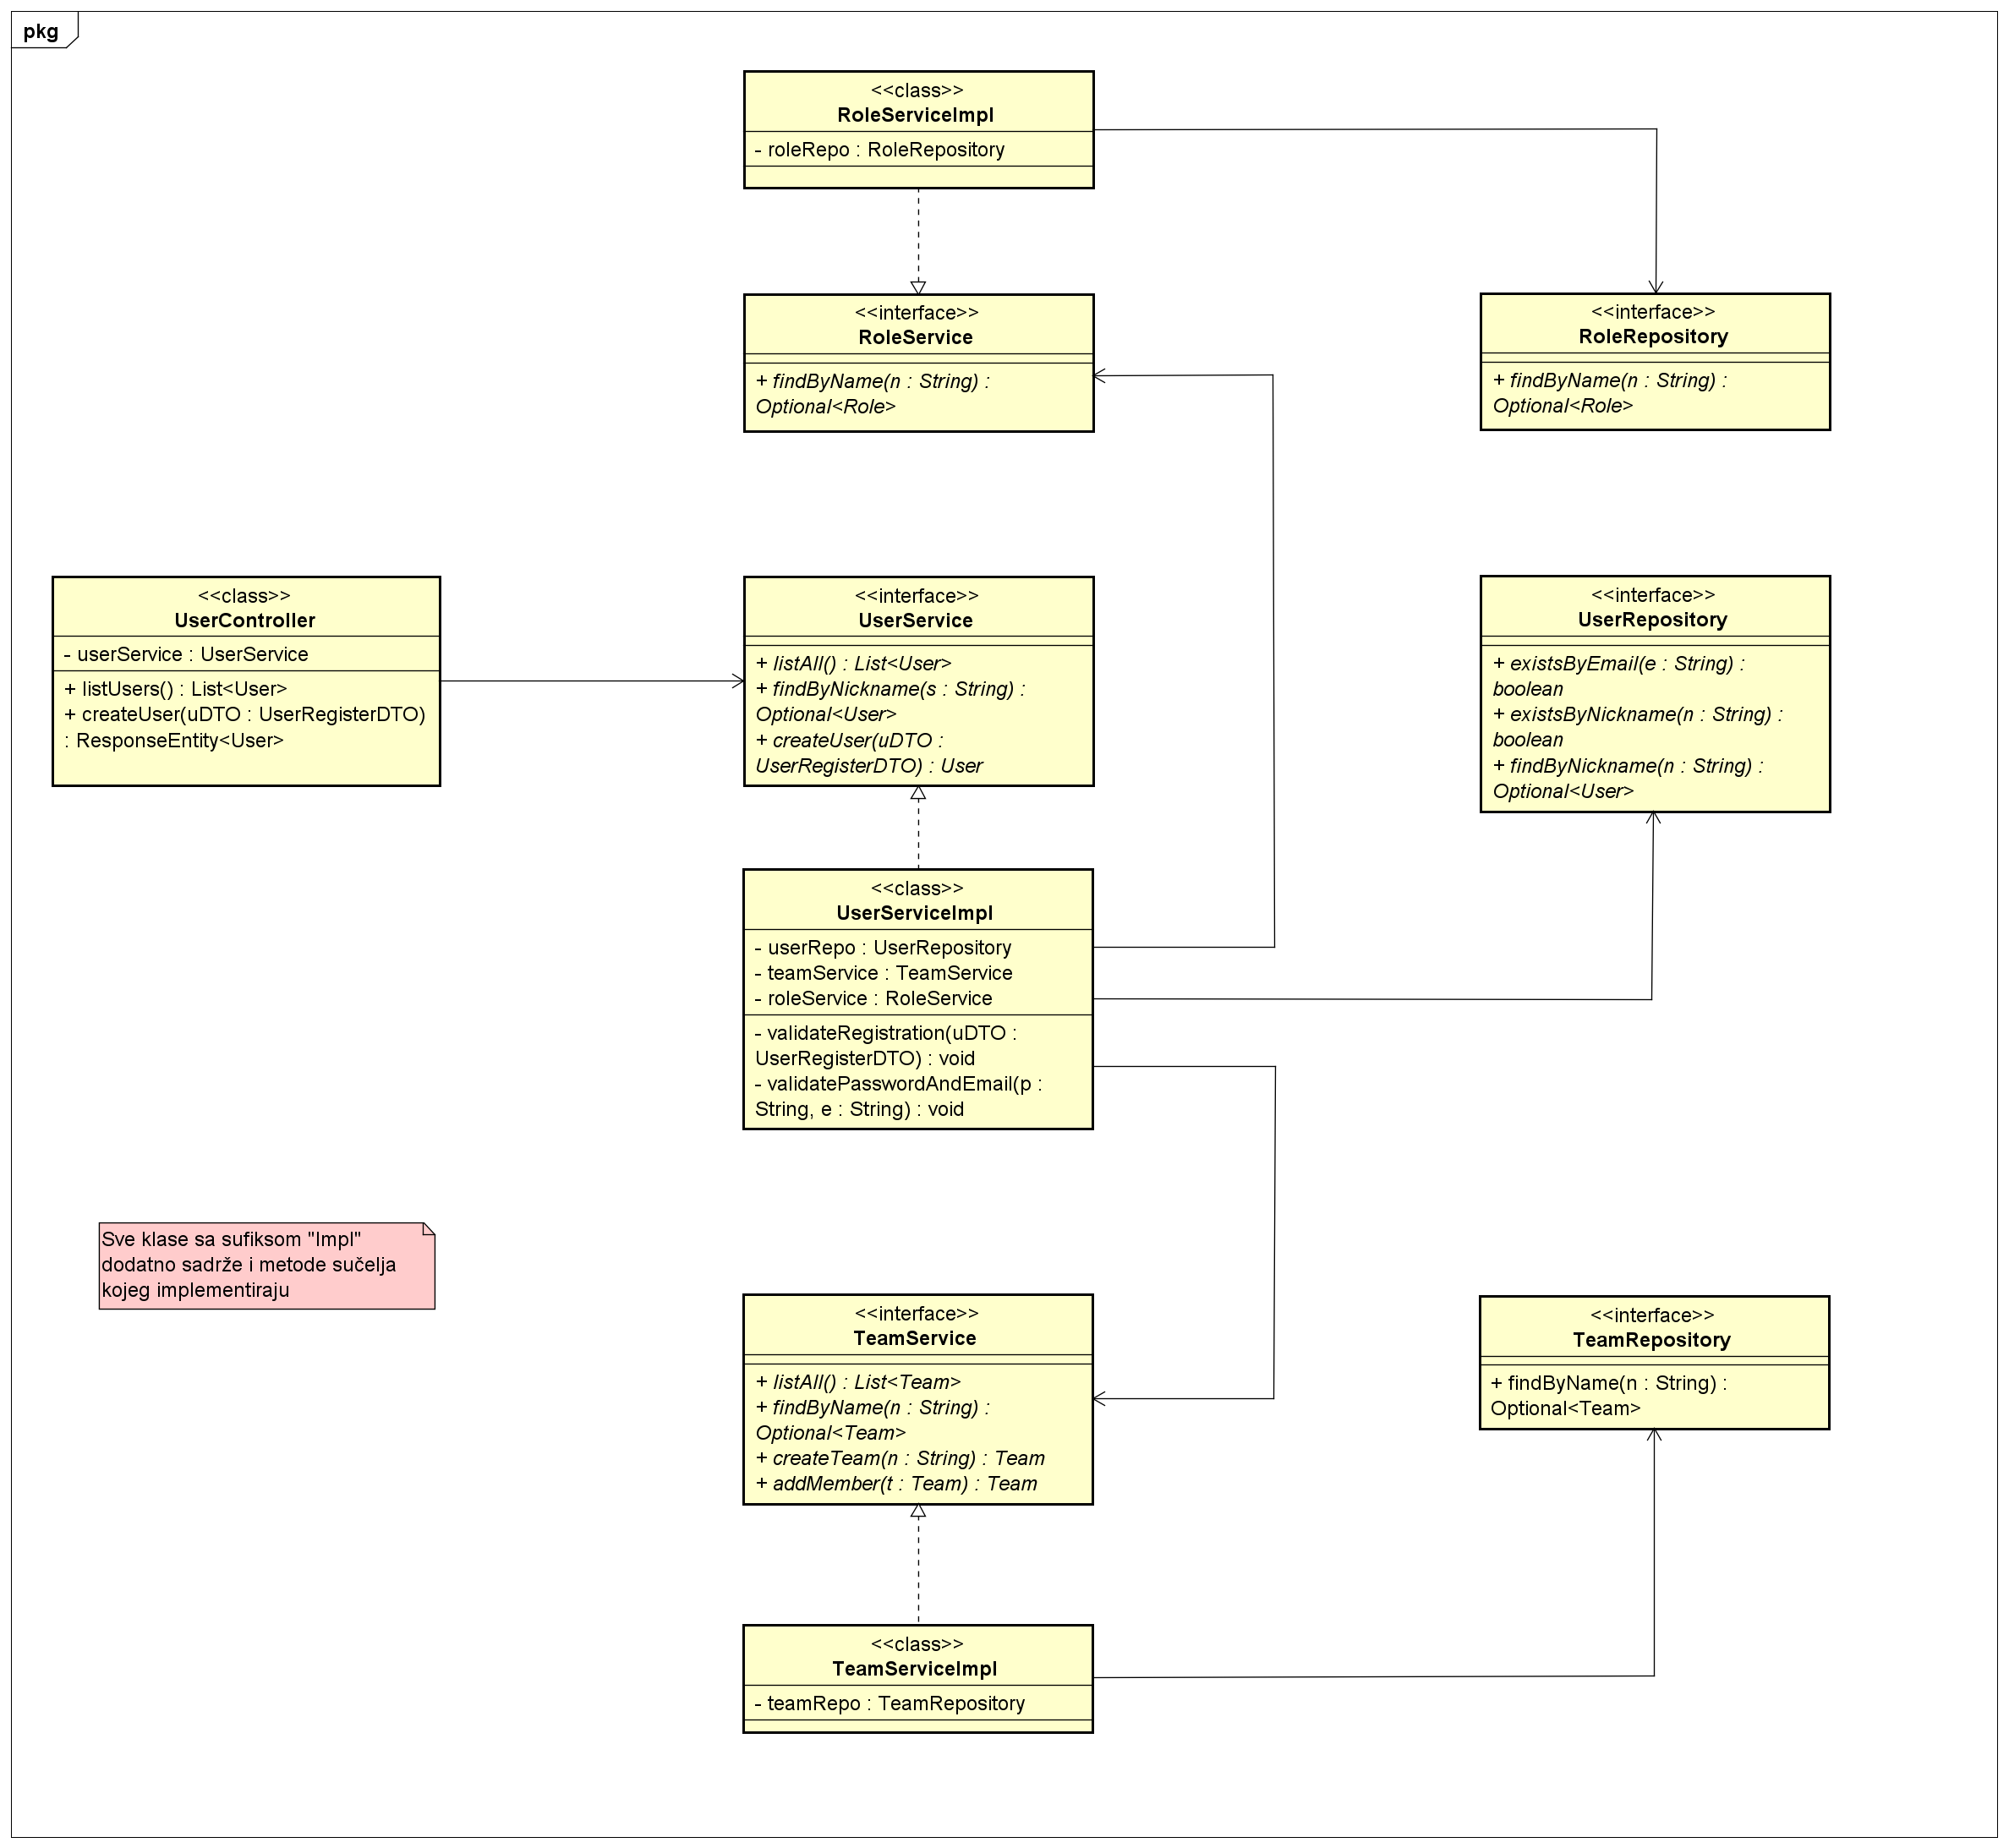
\includegraphics[width=\textwidth]{dijagrami/classDiagram2.PNG} 
				\caption{Dijagram razreda, kontroleri - servisi - repozitoriji}
				\label{fig:classDiagram2}
			\end{figure}
		
			Na slici 4.4 prikazan je dijagram razreda koji prikazuje organizaciju backenda aplikacije podijeljenu u tri sloja. Prvi sloj čini UserController koji prima zahtjeve i korisniku šalje odgovor te ostvaruje komunikaciju sa slojem poslovne logike u kojem se nalaze sučelja UserService, RoleService i TeamService s popisom potrebnih metoda te njihove pripadajuće implementacije - razredi UserServiceImpl, RoleServiceImpl i TeamServiceImpl. Svaki od navedenih razreda ostvaruje vezu sa svojim repozitorijem, a svaki repozitoriji predstavljen je sučeljem koje onda dodatno nasljeđuje sučelje JpaRepository\textless T, ID\textgreater{} radnog okvira Spring Boot za čiju se implementaciju on sam i pobrine.
			\newline\newline
	
			\textbf{\textit{dio 2. revizije}}\\			
			
			\textit{Prilikom druge predaje projekta dijagram razreda i opisi moraju odgovarati stvarnom stanju implementacije}
			
	
			
			\eject
		
		\section{Dijagram stanja}
		
		
		Dijagram stanja opisuje dinamičko ponašanje dijela sustava u vremenu i  modelira situaciju tijekom koje vrijedi određeni skup uvjeta. Na slici je prikazan dijagram stanja koji prikazuje korisničko sučelje prijavljenog korisnika. Nakon prijave, korisnik je preusmjeren na Home stranicu na kojoj može pregledati opis i logo aplikacije. Koristeći navigacijsku traku može odabirati bilo koju od ponuđenih stranica aplikacije i tako mijenjati prikaz, odnosno stanja. Na stranici Account pregledava svoj korisnički profil te ga može ažurirati odabirom uređivanja profila. Odabirom stranice Stats korisnik može pregledati statistiku, a odabere li stranicu Notifications može vidjeti svoje obavijesti i bilo koju od njih dodatno pregledati. Na stranici Events prikazuju se svi aktivni kvizovi, a korisnik ovisno o ulozi koju ima u aplikaciji može izvoditi opisane akcije. Također, ako korisnik ima ulogu administratora može odabrati stranicu Users te blokirati ili dodijeliti administratorska prava ostalim korisnicima aplikacije. Igrač može pregledati stranicu Teams na kojoj su prikazane informacije o njegovoj ekipi, pri čemu može izvršiti akcije pronalaska ili napuštanja tima. Iz svih stanja moguće je odjaviti se iz sustava. 
		
		
		\begin{figure}[H]
			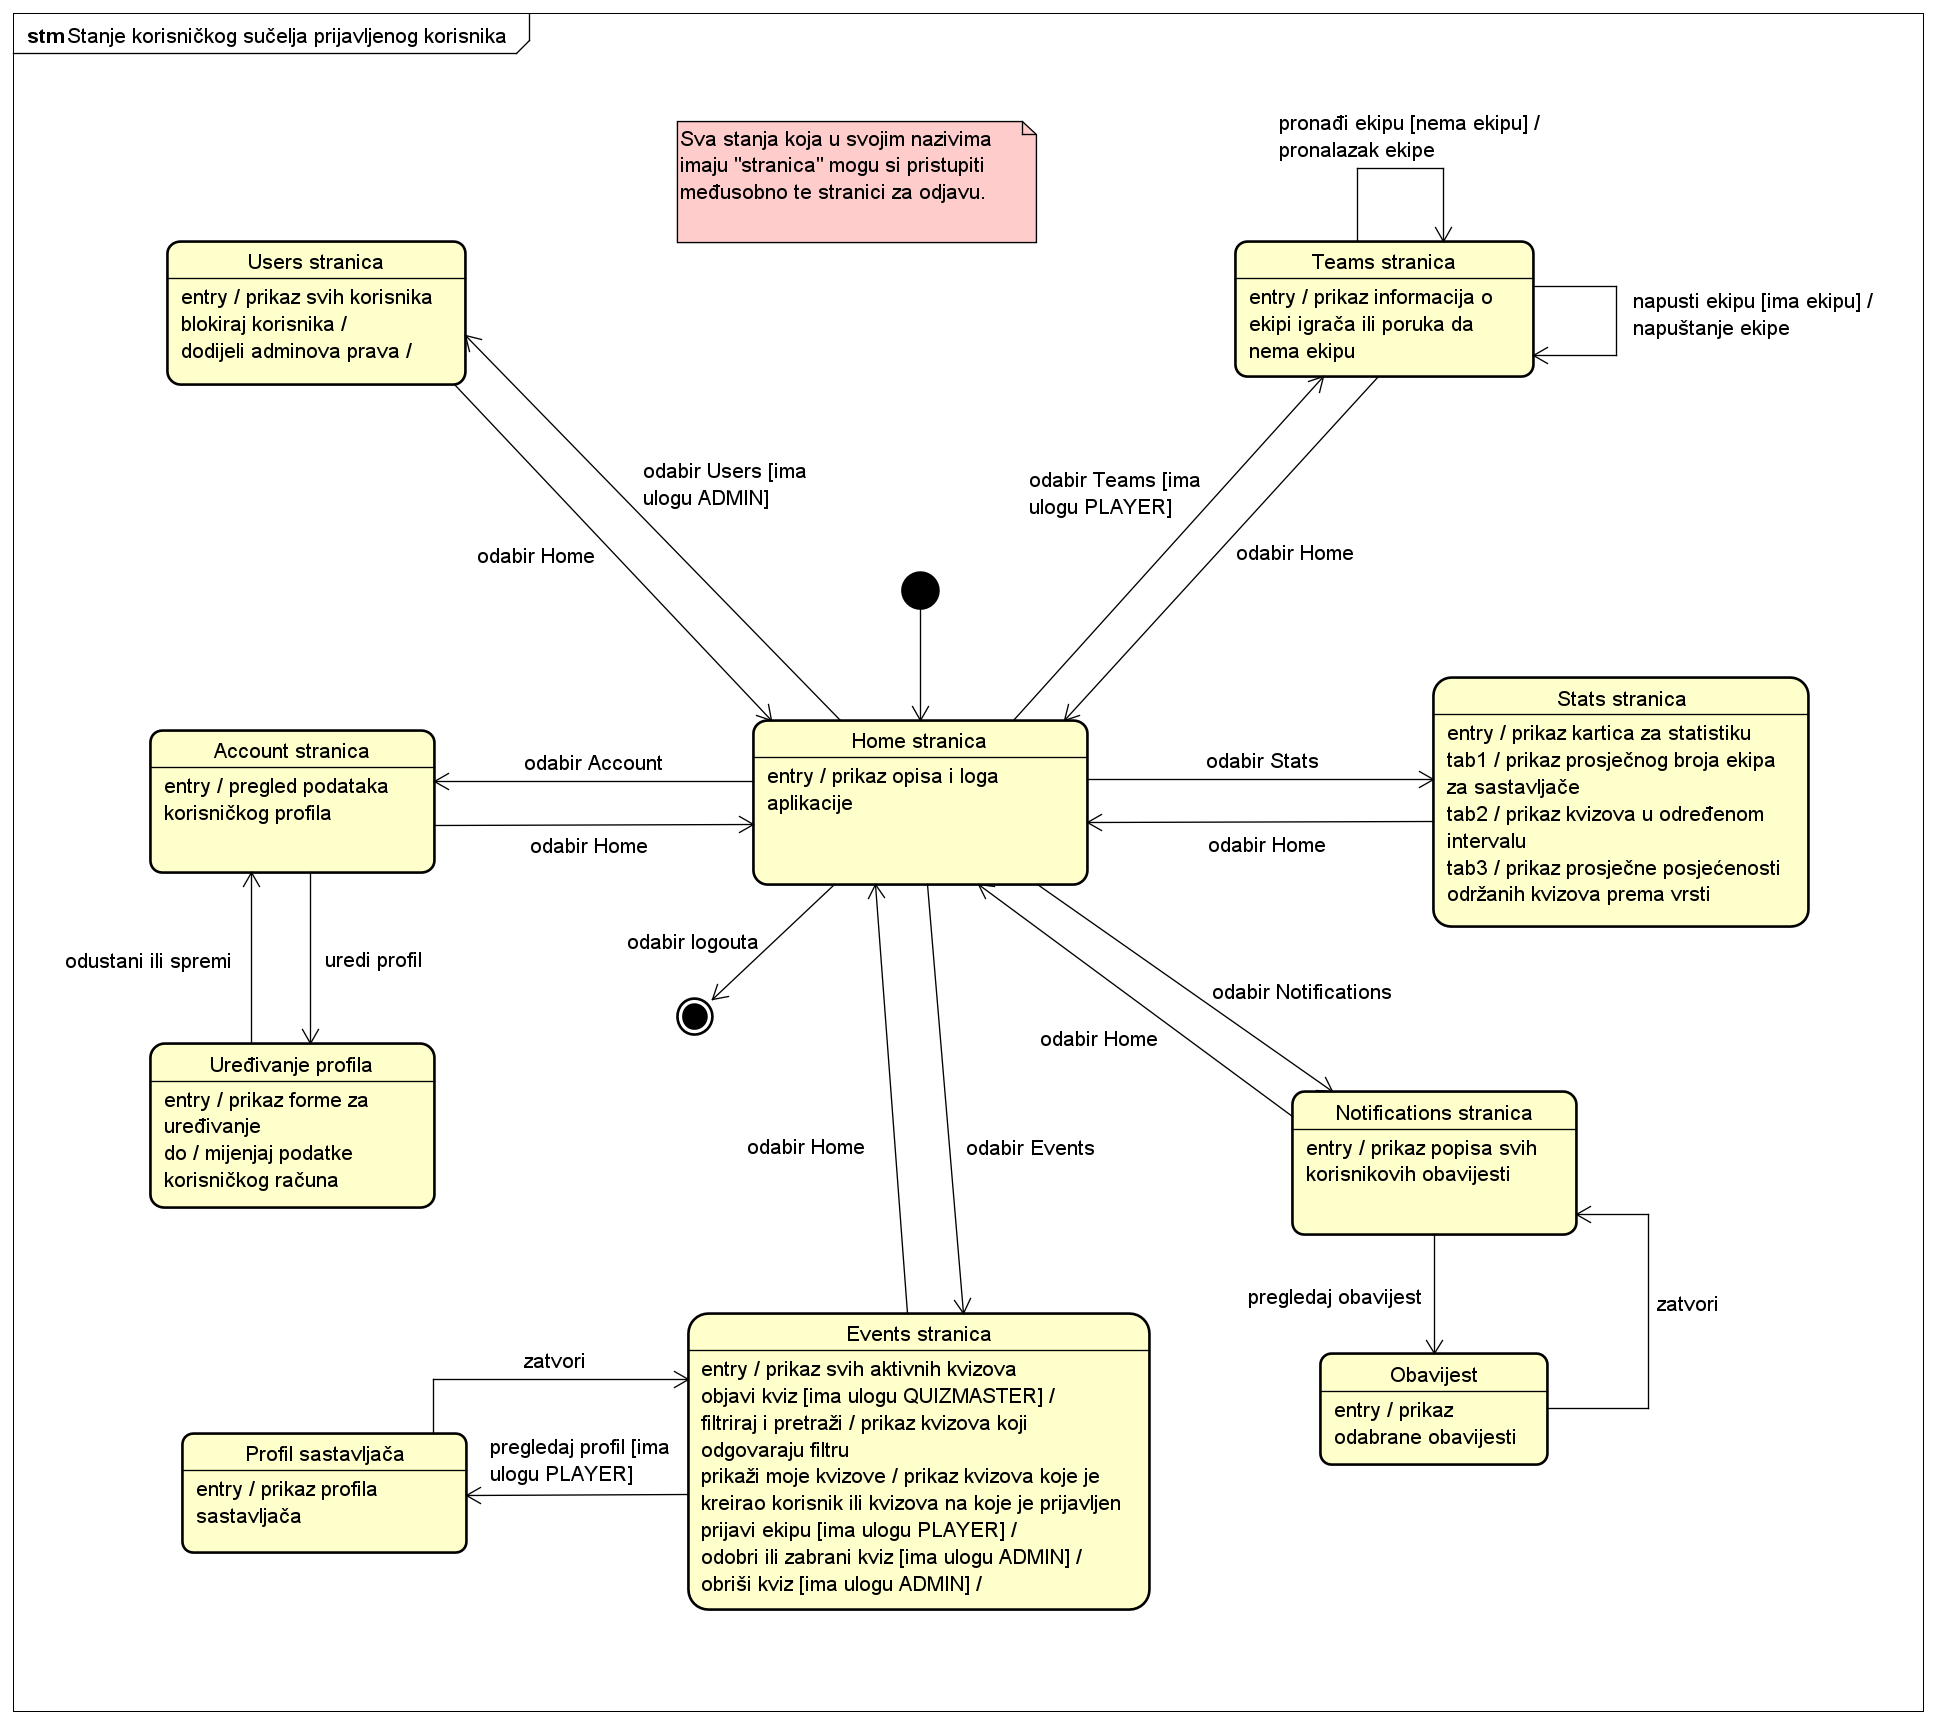
\includegraphics[width=\textwidth]{dijagrami/StatemachineDiagram.PNG} 
			\caption{Dijagram stanja}
			\label{fig:StatemachineDiagram}
		\end{figure}
		
		
		\eject 
		
		\section{Dijagram aktivnosti}
		
		
		Dijagram aktivnosti je ponašajni UML dijagram koji modelira ponašanja nizom akcija, pri čemu se mogu definirati uvjeti prije i nakon njihova izvođenja. Primjenjuje se za modeliranje poslovnih procesa i upravljačkog toka, na primjer toka analize obrazaca uporabe kao što je to i ovdje slučaj. Dijagram na slici prikazuje aktivnost kreiranja pub kviza, a podijeljen je na tri vertikalne particije prema aktorima sustava. Sastavljač kviza prijavljuje se u aplikaciju, nakon čega se provjerava ispravnost unesenih podataka. Ako su podaci neispravni korisnik se vraća na unos podataka, a ako su ispravni preusmjerava se na početnu stranicu. Nakon odabira stranice Events i unosa podataka za kreiranje kviza slijedi evaluacija istih podataka i vraćanje odgovora o njihovoj ispravnosti. Ako su podaci neispravni sastavljač može odustati od kreiranja kviza ili ponovno unijeti podatke. Međutim, ako su uneseni podaci ispravni kviz se kreirao i sprema se u bazu podataka, nakon čega slijedi obavijest o kreiranom kvizu i završavanje s radom.   
		
		\begin{figure}[H]
			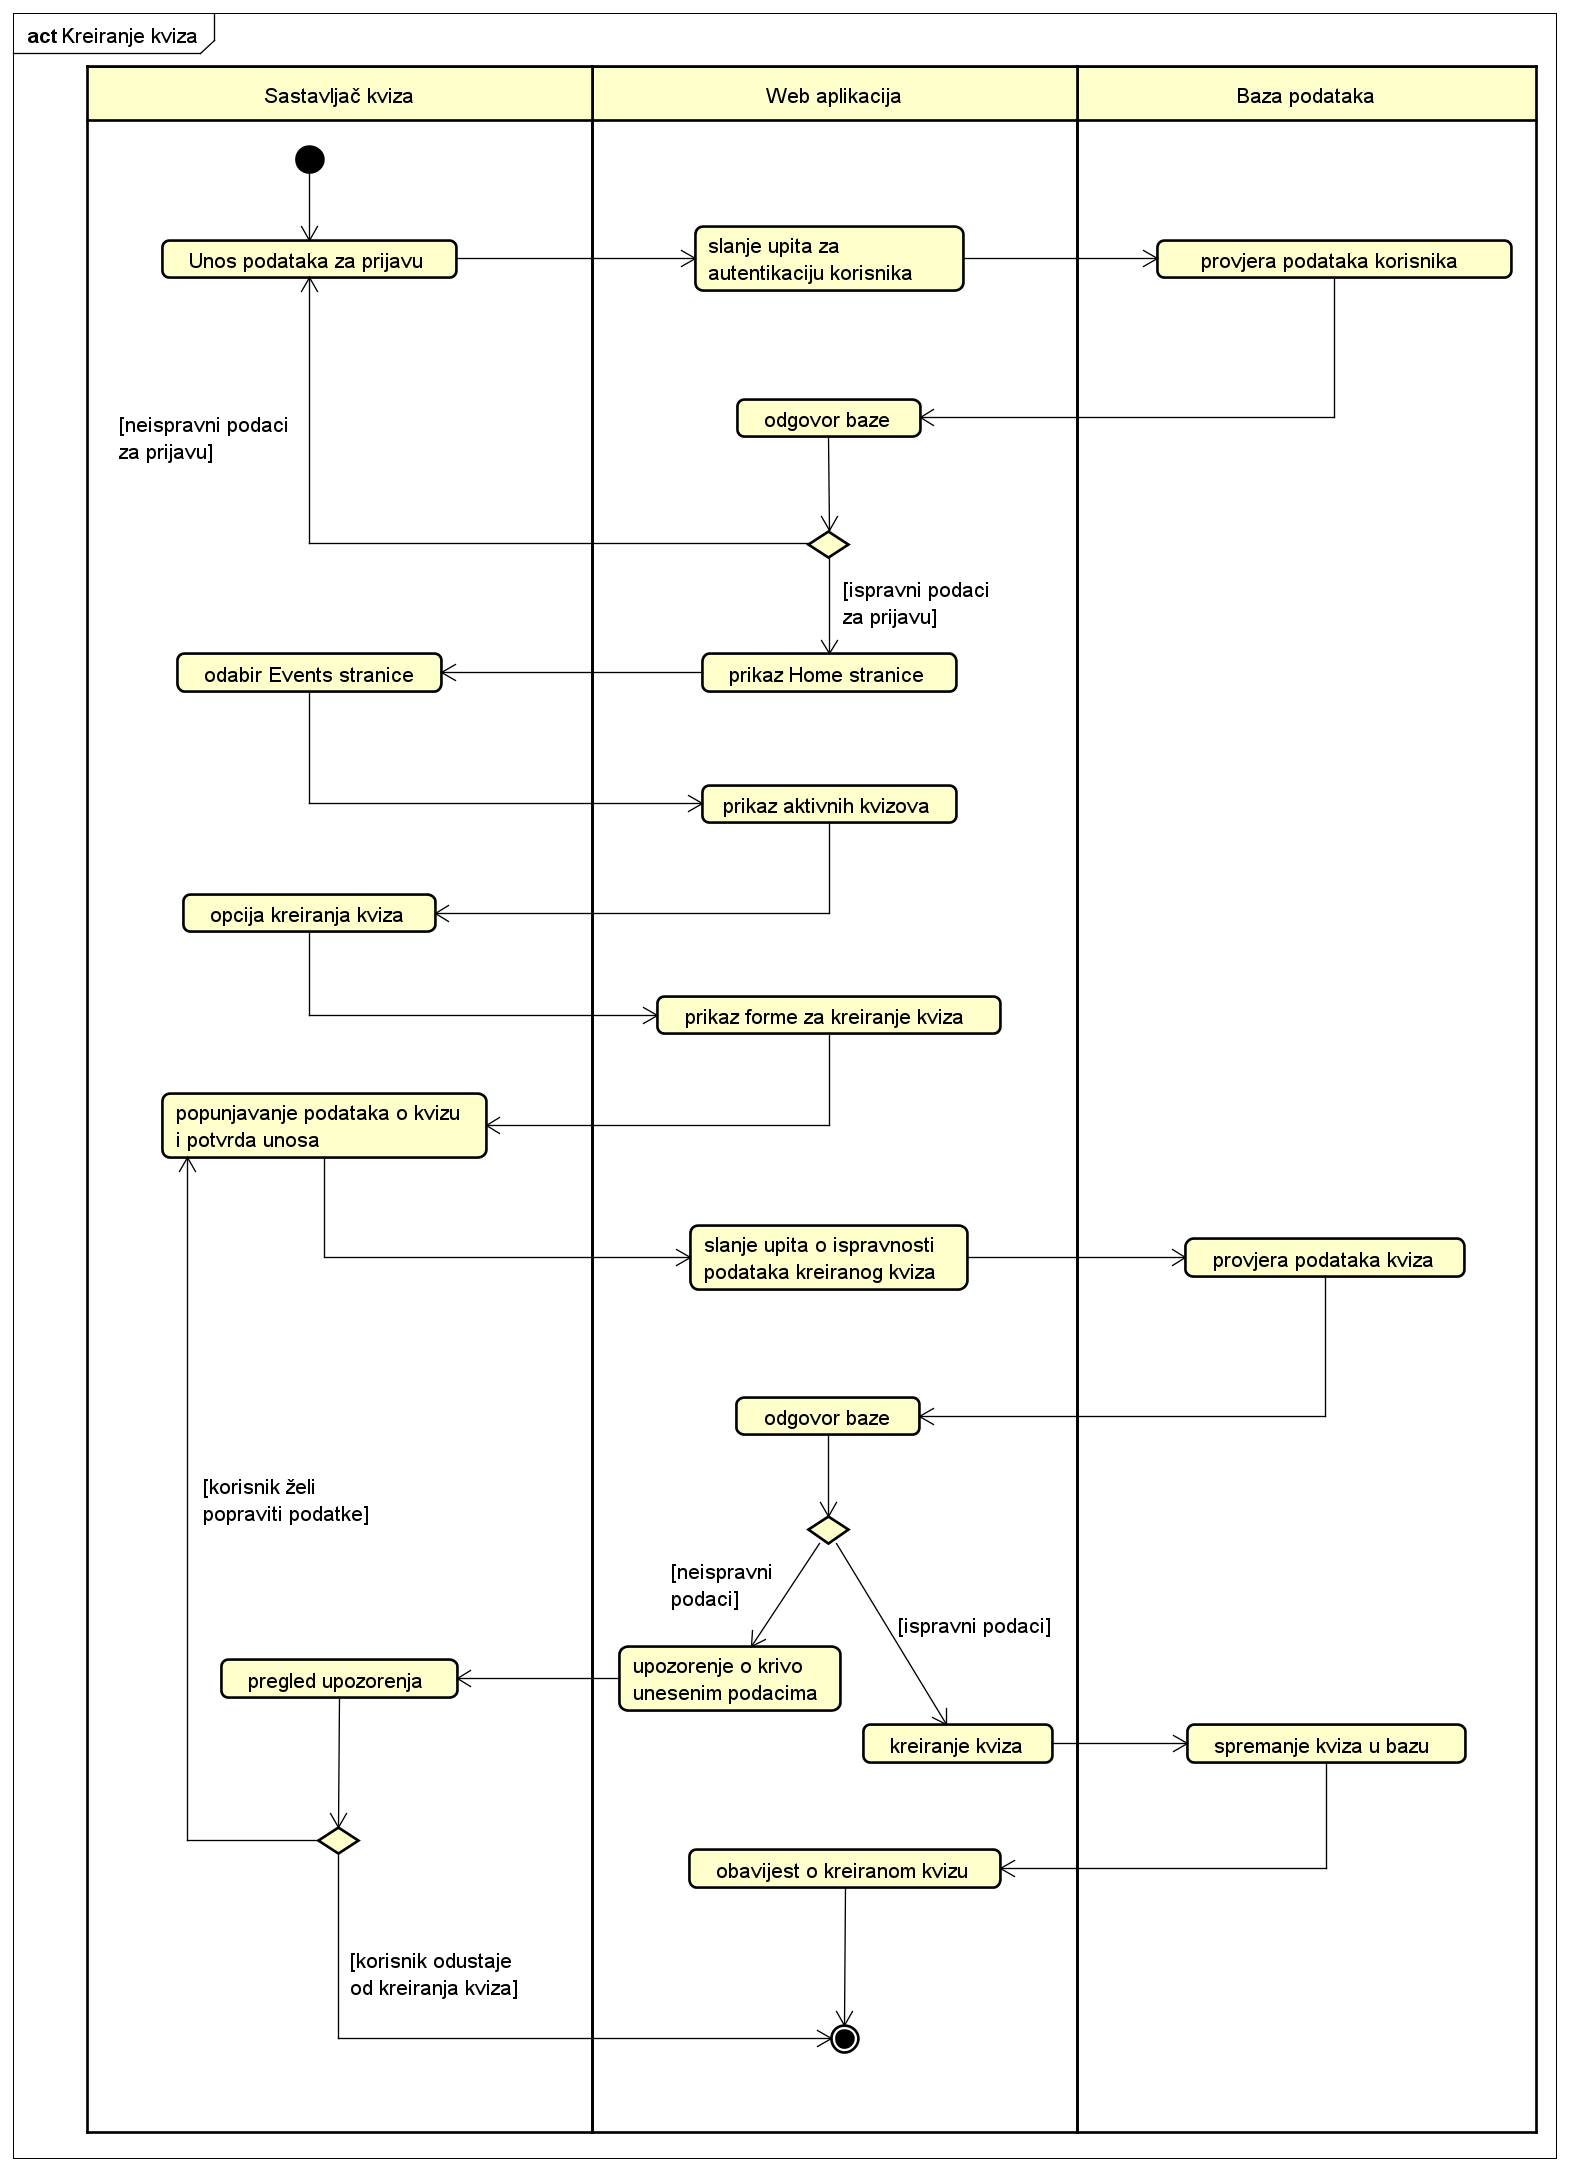
\includegraphics[width=\textwidth]{dijagrami/ActivityDiagram.PNG} 
			\caption{Dijagram aktivnosti}
			\label{fig:ActivityDiagram}
		\end{figure}
		
		\eject
		\section{Dijagram komponenti}
		
			Dijagram komponenti je strukturni statički UML dijagram koji služi za vizualizaciju organizacije i međuovisnosti između implementacijskih komponenata i čini dio specifikacije arhitekture programske potpore. Za pristup sustavu koriste se dva sučelja. Preko sučelja I$\_$HTML$\_$CSS$\_$JS dohvaćaju se HTML, CSS i JS datoteke koje pripadaju frontend dijelu aplikacije. Komponenta Router na upit preko URL-a odlučuje koja će se datoteka poslužiti na sučelje. Frontend se sastoji od JavaScript datoteka koje su raspoređene po komponentama nazvanim prema stranicama aplikacije. Sve te datoteke ovise o React biblioteci iz koje dohvaćaju već gotove komponente poput formi i slično. Preko REST$\_$API sučelja pristupa se komponenti Controller koja poslužuje podatke iz backend dijela aplikacije. Repository je zadužen za dohvaćanje podataka iz tablica baze podataka pomoću SQL upita, a koristeći pritom SQL$\_$API sučelje. React-view komponenta preko dostupnih sučelja komunicira s aplikacijom te ovisno o korisnikovim akcijama osvježava prikaz i dohvaća nove podatke ili datoteke.
			
			\begin{figure}[H]
				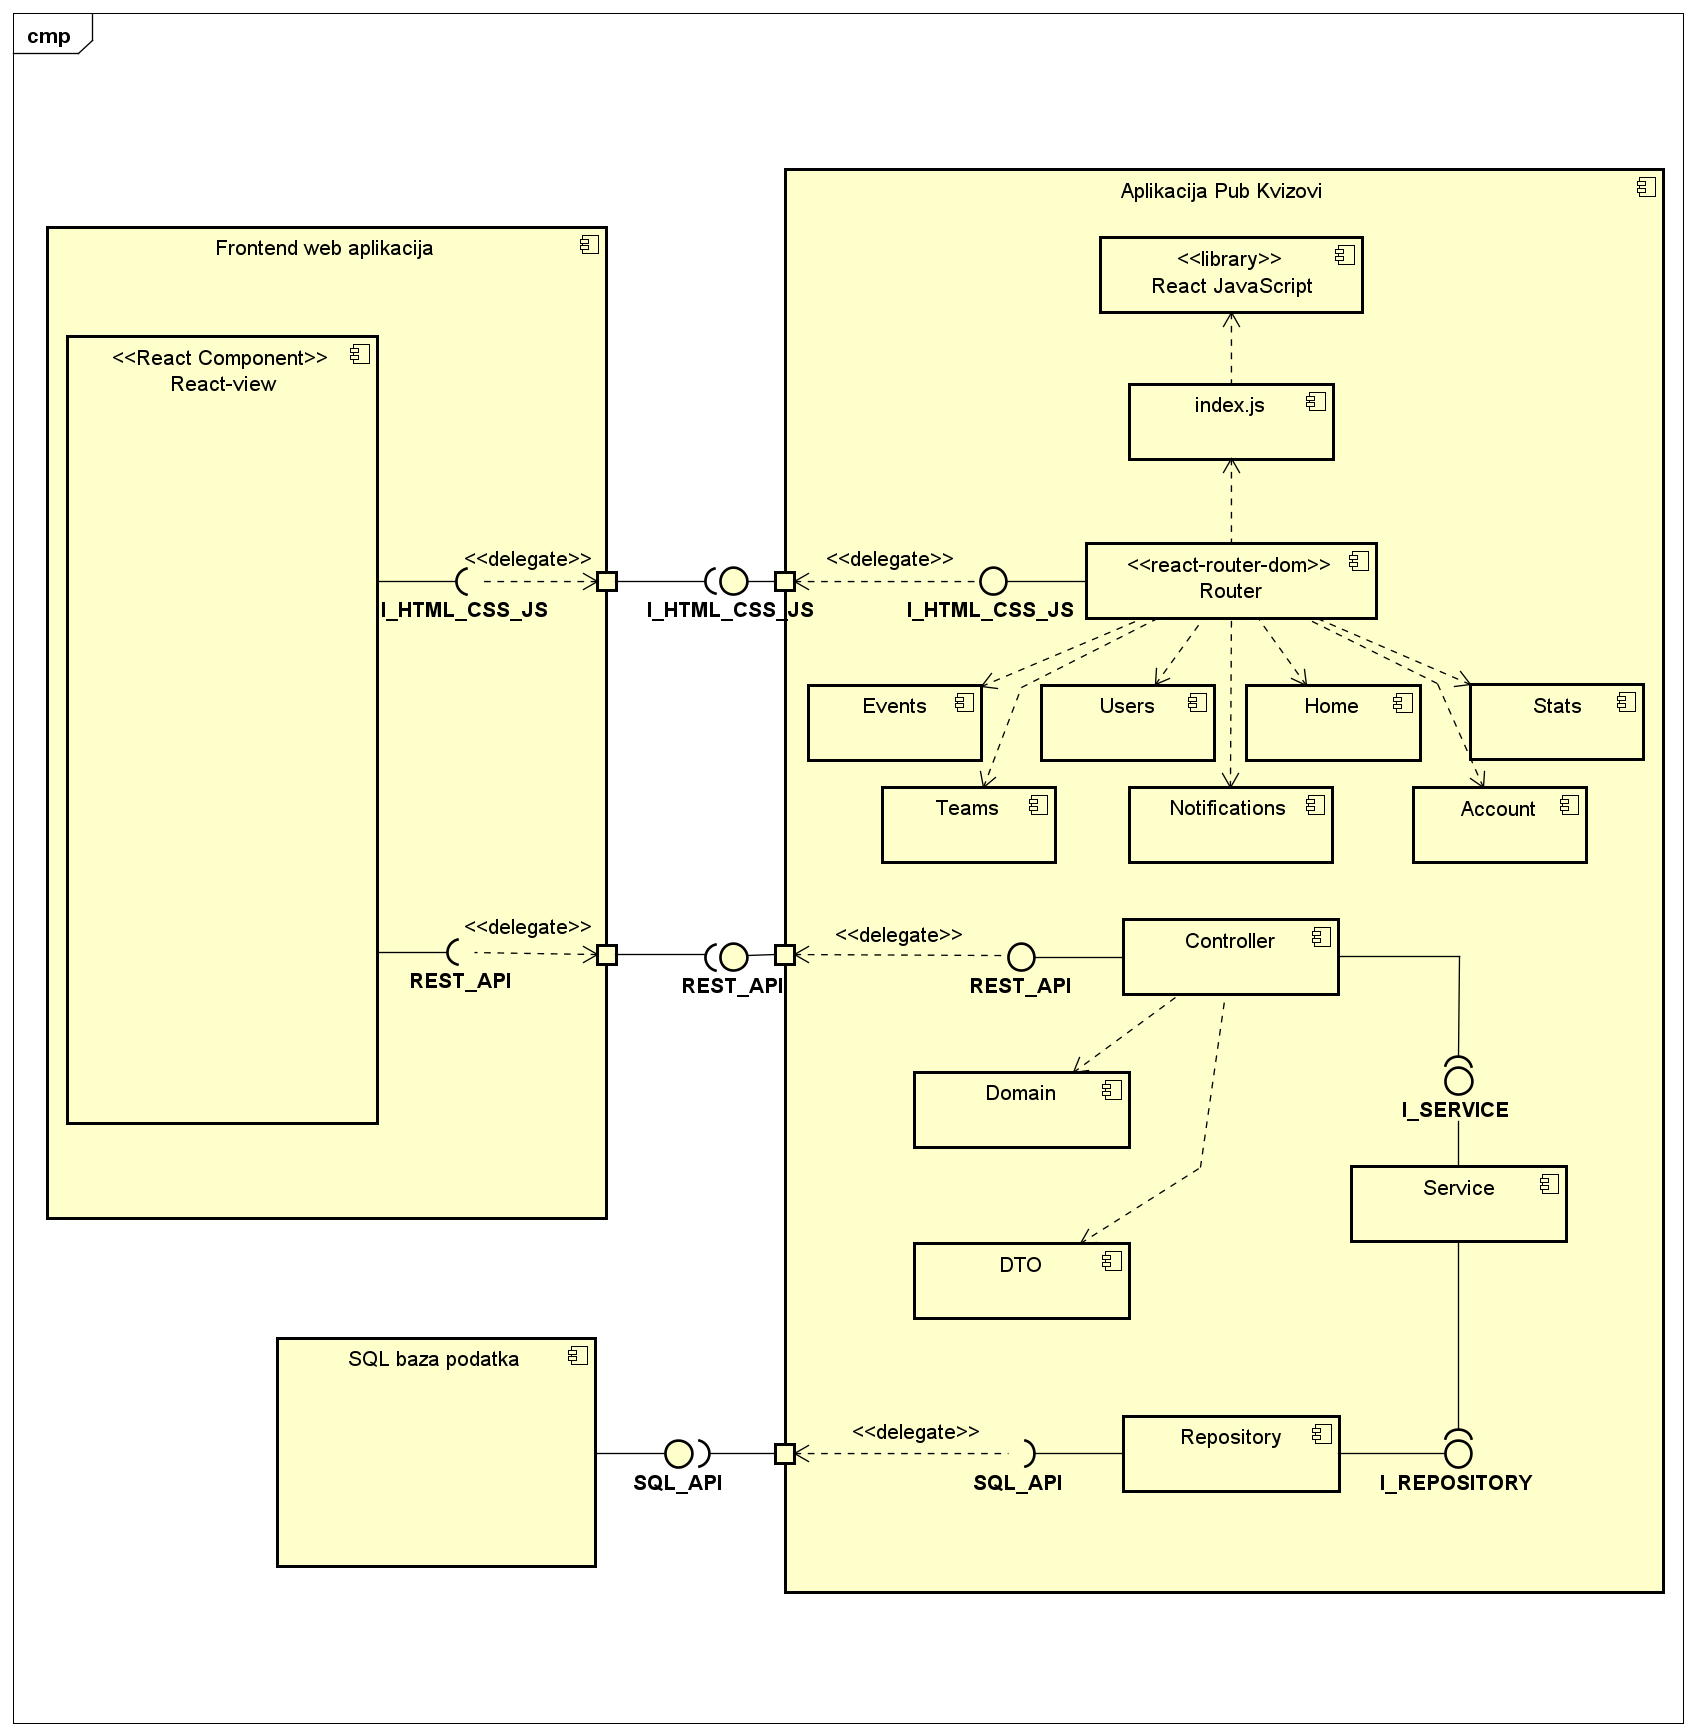
\includegraphics[width=\textwidth]{dijagrami/ComponentDiagram.PNG} 
				\caption{Dijagram komponenti}
				\label{fig:ComponentDiagram}
			\end{figure}
		
	